\documentclass[a4paper, english]{article}
\usepackage{graphicx,color,eurosym,latexsym}
\usepackage{listings}
\usepackage{pst-all}
\usepackage{algorithmic,algorithm}
\lstset{columns=fixed,basicstyle=\ttfamily,numbers=left,numberstyle=\tiny,stepnumber=5,breaklines=true}
\usepackage{times}
\usepackage{babel}
\usepackage[useregional]{datetime2}
\usepackage[round]{natbib}
\bibliographystyle{plainnat}
\oddsidemargin=0cm
\evensidemargin=0cm
\newcommand{\be}{\begin{enumerate}}
\newcommand{\ee}{\end{enumerate}}
\newcommand{\bi}{\begin{itemize}}
\newcommand{\ei}{\end{itemize}}
\newcommand{\I}{\item}
\newcommand{\ty}{\texttt}
\textwidth=16cm
\textheight=23cm
\begin{document}
\title{\ty{Epos} v1.1
: Estimating Population Sizes and Allele Ages from
  Site Frequency Spectra}
\author{Bernhard Haubold\\\small Max-Planck-Institute for Evolutionary
  Biology, Pl\"on, Germany}
\date{\input{date}}
\maketitle

\tableofcontents

\section{Introduction} 
The software package \ty{epos} contains two programs, \ty{epos}
itself and the auxiliary program \ty{epos2ages}. \ty{Epos} estimates historical population
sizes and \ty{epos2ages} transforms them into allele ages. In this document I first
explain \ty{epos} and how to build the programs of the package. Then I
give a tutorial-style introduction to their usage.

\ty{Epos} takes site frequency spectra as input. A site frequency
spectrum is computed from a haplotype sample. For example, Table~\ref{tab:hap}
shows a sample of $n=4$ haplotypes, $h_1, h_2,...,h_4$, with $S=8$
segregating (polymorphic) sites, $s_1, s_2,...,s_8$. Each segregating
site consists of a column of four zeros and ones, where zero indicates
the ancestral state and one a mutation. We can count the number of
sites where one, two, or three haplotypes are mutated. This is called
the site frequency spectrum (SFS) of the sample, and
Table~\ref{tab:sfs}A shows the spectrum for our example data. There
are seven mutations affecting a single haplotype (singletons), zero
mutations affecting two haplotypes (doubletons), and one mutation
affecting three haplotypes (tripleton).
\begin{table}
  \caption{Four example haplotypes}\label{tab:hap}
  \begin{center}
    \begin{tabular}{lcccccccc}\hline
haplotype   &   $s_1$ & $s_2$ & $s_3$ & $s_4$ & $s_5$ & $s_6$ & $s_7$ & $s_8$\\\hline
$h_1$ &      \ty{1} & \ty{0} & \ty{0} & \ty{0} & \ty{0} & \ty{0} & \ty{0} & \ty{0}\\
$h_2$ &      \ty{0} & \ty{1} & \ty{0} & \ty{0} & \ty{1} & \ty{0} & \ty{0} & \ty{1}\\
$h_3$ &      \ty{0} & \ty{1} & \ty{0} & \ty{1} & \ty{0} & \ty{1} & \ty{0} & \ty{0}\\
$h_4$ &      \ty{0} & \ty{1} & \ty{1} & \ty{0} & \ty{0} & \ty{0} & \ty{1} &
      \ty{0}\\\hline
      \end{tabular}
  \end{center}
\end{table}
In many empirical data sets it is not possible to distinguish between
segregating sites with $r$ mutant alleles and those with $n-r$
mutant alleles. In this case the spectrum is called \textit{folded} and
consists of the
number of sites affecting $r$ haplotypes plus the number of sites
affecting $n-r$ haplotypes. Table~\ref{tab:hap}B shows the folded
version of the spectrum in Table~\ref{tab:hap}A: The singleton
category now consists of the sum of unfolded singletons and
tripletons, while the number of doubletons
remains unchanged.

\begin{table}
  \caption{Folded (\textbf{A}) and unfolded (\textbf{B}) site
    frequency spectrum corresponding to the haplotype sample shown in Table~\ref{tab:hap}}\label{tab:sfs}
  \begin{center}
  \begin{tabular}{cc}
    \textbf{A} & \textbf{B}\\
    \begin{tabular}{cc}
      \hline
      $r$ & $f(r)$\\\hline
      1 & 7\\
      2 & 0\\
      3 & 1\\\hline
    \end{tabular}
    &
    \begin{tabular}{cc}
      \hline
      $r$ & $f(r)$\\\hline
      1 & 8\\
      2 & 0\\
      \hline
    \end{tabular}
  \end{tabular}
  \end{center}
\end{table}

\ty{Epos} implements theory by \cite{lyn19:inf}, which I briefly
summarize here. Consider the coalescent for $n$ haplotypes,
Figure~\ref{fig:coa} shows an example for $n=4$ haplotypes. Any such
coalescent can be divided into levels $2, 3,...,n$, where a level,
$\ell$, is marked by the coalescence event that reduces the number of
lineages from $\ell+1$ to $\ell$. The time intervals $T_i, 2\le i\le
n-1$, denote the segments of the coalescent with $i$ lineages. For each $T_i$ \ty{epos}
can calculate a corresponding number of diploid individuals making up
the population, $N_i$. Unfortunately,
for larger samples the computation of all $N_i$ invariably
returns negative population sizes. So instead of allowing the
population size to change at every coalescence event, we pick a subset
of levels encapsulating the most important size changes.

\begin{figure}
  \begin{center}
    \begin{pspicture}(-1.5,0)(2.5,2.75)
  \psset{xunit=0.25,yunit=0.25}
  \rput( 0.00, 0.00){\Rnode{1}{$h_1$}}
  \rput( 3.33, 0.00){\Rnode{2}{$h_2$}}
  \rput( 6.67, 0.00){\Rnode{3}{$h_3$}}
  \rput(10.00, 0.00){\Rnode{4}{$h_4$}}
  \rput( 1.67, 3.09){\Rnode{5}{}}
  \rput( 5.00, 2.43){\Rnode{6}{}}
  \rput( 8.33, 8.57){\Rnode{7}{}}
  
  \ncline[nodesepA=2pt]{1}{5}
  \ncline[nodesepA=2pt]{2}{6}
  \ncline[nodesepA=2pt]{3}{6}
  \ncline{6}{5}
  \ncline{5}{7}
  \ncline[nodesepA=2pt]{4}{7}

  \rput(-2, 11){$T_i$, $N_i$}
  \rput(12, 11){Level}

  \rput(-2, 0.00){\Rnode{ 8}{}}
  \rput(-2, 2.43){\Rnode{ 9}{}}
  \rput(-2, 3.09){\Rnode{10}{}}
  \rput(-2, 8.57){\Rnode{11}{}}

  \rput(12, 0.00){\Rnode{12}{ 5}}
  \rput(13, 2.43){\Rnode{13}{ 4}}
  \rput(12, 3.09){\Rnode{14}{ 3}}
  \rput(12, 8.57){\Rnode{15}{ 2}}

  \ncline[linestyle=dotted]{8}{12}
  \ncline[linestyle=dotted]{9}{13}
  \ncline[linestyle=dotted]{10}{14}
  \ncline[linestyle=dotted]{11}{15}

  \ncline{<->}{8}{9}\naput{$T_4, N_4$}
  \ncline{<->}{9}{10}\naput{$T_3, N_3$}
  \ncline{<->}{10}{11}\naput{$T_2, N_2$}
\end{pspicture}

  \end{center}
  \caption{A coalescent for $n=4$ haplotypes to illustrate the time
    intervals, $T_i$, the corresponding population sizes, $N_i$, and
    the \emph{levels} in the tree.}\label{fig:coa}
\end{figure}

Each combination of levels must contain level 2, the root. If no
further level is added, $N_2$ is computed, the population size for the
whole coalescent. Similarly, breakpoints at levels 2 and 4 would mean
that there is one population size for $T_2$ and $T_3$, and another
for $T_4$.

So, given a combination of levels, the population sizes are computed
with the proviso that negative values are set to the smallest possible
population size, $N=1$. For each combination of levels and population
sizes, the log-likelihood of observing the input site frequency
spectrum is calculated \citep{lyn19:inf}. We now need an efficient a method
for maximizing this likelihood.

The starting point is always a single level, $m=1$, the root at level
2. Then all level pairs $(2,3), (2,4),...,(2,n)$ are examined and the
most likely combination picked. If this improves the likelihood by at
least 2 units, the number of levels is increased to $m=3$ and the
search repeats. Algorithm~\ref{alg:epo} summarizes this strategy. The
function \ty{nextConfig} in line 7 hides the details of how the next
configuration is picked. I have implemented a \emph{greedy} and an
\emph{exhaustive} strategy. Under the greedy strategy, the best
configuration of breakpoints found in round $m$ is retained in round
$m+1$ and a single new breakpoint is added. Under the exhaustive
strategy, all ${n-1\choose m-2}$ possible combinations of breakpoints
are investigated in each round. Unfortunately, for large samples, this
number quickly leads to unacceptable run times and hence greedy is the
default. The greedy and exhaustive search strategies are explained
further in the Tutorial in Section~\ref{sec:tut}, where I also apply
\ty{epos} to real site frequency spectra before also explaining
\ty{epos2ages}.

\begin{algorithm}
  \caption{Searching for break points in the coalescent}\label{alg:epo}
  \begin{algorithmic}[1]
  \REQUIRE{$n$} \COMMENT{Sample size}
  \REQUIRE{$\mathrm{f}$} \COMMENT{Array of $n-1$ or $n/2$ site frequencies, the
  unfolded or folded site frequency spectrum, SFS}
  \ENSURE{$m$} \COMMENT{Number of estimated population sizes}
  \ENSURE{$\mathrm{k}$} \COMMENT{Array of $m$ population size change points}
  \ENSURE{$\mathrm{N}$} \COMMENT{Array of $m$ population sizes at
    change points $\mathrm{k}[i], i=1,2,...,m$}
  \STATE{$m\leftarrow 1$} \COMMENT{Initialize to one population size...}
  \STATE{$\mathrm{k}[m]\leftarrow 2$} \COMMENT{...which starts at the root}
  \STATE{$\mathrm{N}\leftarrow \ty{popSizes}(m, \mathrm{k}, \mathrm{f})$}
  \COMMENT{Size of constant population}
  \STATE{$l\leftarrow\ty{likelihood}(\mathrm{N}, m, \mathrm{k},
    \mathrm{f})$} \COMMENT{Likelihood of population size given the SFS}
  \STATE{$l_{\rm a}\leftarrow l$} \COMMENT{The initial likelihood is
    also the maximum}
  \FOR{$m\leftarrow 2$ to $n$} 
     \WHILE{$(\mathrm{k}'\leftarrow\ty{nextConfig}(m, n))\ne\mathrm{null}$} 
        \STATE{$\mathrm{N}'\leftarrow\ty{popSizes}(m, \mathrm{k}',
          \mathrm{f})$}
        \STATE{$l'\leftarrow\ty{likelihood}(\mathrm{N}', m, \mathrm{k}',
          \mathrm{f})$}
        \IF{$l'>l_{\rm a}$}
           \STATE{$\mathrm{k}_{\rm a}\leftarrow\mathrm{k}'$}
           \STATE{$\mathrm{N}_{\rm a}\leftarrow\mathrm{N}'$}
           \STATE{$l_{\rm a}\leftarrow l'$}
        \ENDIF
     \ENDWHILE
     \IF{$l_{\rm a} < l+2$}
        \STATE{$\ty{report}(\mathrm{N}, \mathrm{k}, m-1)$}
        \STATE{$\ty{break}$}
     \ENDIF
     \STATE{$\mathrm{k}\leftarrow \mathrm{k}_{\rm a}$}
     \STATE{$\mathrm{N}\leftarrow \mathrm{N}_{\rm a}$}
     \STATE{$l\leftarrow l_{\rm a}$}
  \ENDFOR
\end{algorithmic}

\end{algorithm}

\section{Getting Started}
The \ty{epos} package was written in C and Go on a computer running
Linux. It depends on
two libraries, the Gnu Scientific Library
(\ty{lgsl}), and the Basic Linear Algebra Subprograms (\ty{lblas}). 
Please contact \ty{haubold@evolbio.mpg.de} if there are any problems with the program.
\bi
\I Obtain the package
\begin{verbatim}
git clone https://www.github.com/evolbioinf/epos
\end{verbatim}
\I Change into the directory just downloaded
\begin{verbatim}
cd epos
\end{verbatim}
and make the programs
\begin{verbatim}
make
\end{verbatim}
\I Test the programs
\begin{verbatim}
make test
\end{verbatim}
which takes approximately one minute.
\I The executables are located in the
directory \ty{build}. Place them in your \ty{PATH}.
\I  Make the documentation
\begin{verbatim}
make doc
\end{verbatim}
This calls the typesetting program \ty{latex}, so please make sure it
is installed before entering this command. The typeset documentation is located
in
\begin{verbatim}
doc/epos.pdf
\end{verbatim}
\ei

\section{Tutorial}\label{sec:tut}
\subsection{\ty{Epos}}
I first explain how to test \ty{epos} using simulated data, and then
analyze real data.
\subsubsection*{Simulated Data}
\ty{Epos} was developed for estimating variable population
sizes. Nevertheless, we begin with simulated constant-size
scenarios before generating samples under models with varying population
sizes.
\paragraph{Constant Population Size}
\begin{itemize}
\item First, take a look at one of the simulated data sets supplied
  with \ty{epos}:
\begin{verbatim}
cat data/testF.dat
#r      f[r]
1       9526
2       3998
3       2315
4       1487
5       1075
6       873
7       689
8       570
9       567
10      627
11      547
12      605
13      460
14      573
15      236
\end{verbatim}
It is a folded data set, so the sample size $n=30$.
\item Let's analyze it using the command
\begin{verbatim}
epos -l 1e7 -u 1.2e-8 data/testF.dat 
\end{verbatim}
where \ty{-l 1e7} indicates that 10 Mb of sequence were surveyed and
$\mu=1.2\times 10^{-8}$ is the mutation rate per site per generation. The result of this command is
\begin{verbatim}
#InputFile: data/testF.dat
#Polymorphic sites surveyed:      24384
#Monomorphic sites surveyed:    9975616
#m = 1; maximum Log(Likelihood):   -1719.151896 {2}
#m = 2; maximum Log(Likelihood):    -106.137405 {2,11}
#m = 3; maximum Log(Likelihood):    -104.753557 {2,4,11}
#Final Log(Likelihood):             -106.137405
#d^2: 0.00262777
#Level  T[Level]        N[Level]
11      6.69e+03        2.51e+04
2       3.45e+04        7.73e+03
\end{verbatim}
\ty{Epos} prints intermediate configurations of $m$ breakpoints: As
already described in Algorithm~\ref{alg:epo}, it starts with a single
breakpoint, $m=1$, the root at at level 2. The root level must always
be present and the population size starting there extends to the next
breakpoint printed, or, if there is none as in this case, the leaves
of the coalescent. The log-likelihood of the input site frequency
spectrum given the best-fitting constant population size is
-1719.15. In the next round, $m=2$, one new breakpoint is added at
level 11. The log-likelihood increases to -106.14, which is 
1613 log-units greater than the previous log-likelihood. As the minimum
improvement is 2 log-units, the search is continued in round
$m=3$. The breakpoint at level 11 from the previous round is retained
and the next best breakpoint, level 4, is added. The log-likelihood
grows by roughly one units, so the search is abandoned and the
population sizes for the levels 2 and 11 are printed, \ty{N[Level]}. This
search strategy is \emph{greedy}, because it cannot revise the level
configurations found in previous rounds.
\item Instead of searching for the optimal set of breakpoints, these
  can be supplied in the same notation as used for the intermediate
  results using the \texttt{-L} option.
\begin{verbatim}
epos -l 1e7 -u 1.2e-8 -L 2,4,11 data/testF.dat 
#InputFile: data/testF.dat
#Polymorphic sites surveyed:      24384
#Monomorphic sites surveyed:    9975616
#Final Log(Likelihood):             -104.753557
#d^2: 0.00249224
#Level  T[Level]        N[Level]
11      6.80e+03        2.55e+04
4       1.32e+04        6.84e+03
2       3.51e+04        8.23e+03
\end{verbatim}
\item In addition to the population size at each level added to the model, \ty{epos}
  prints the time of the levels in generations, \ty{T[Level]}. If we call $T_k$ the
  time the coalescent spends with $k$ lines, then
  \[
  \ty{T[Level]} = \sum_{k=\ty{Level}}^n E[T_k],
    \]
  where $N_k$ is the population size during $T_k$,
  allows the computation of \ty{T[Level]} as a simple function of the
  population size.
\item In addition to the log-likelihood, a goodness-of-fit measure is
  printed, $d^2$, as suggested by \cite{lap17:acc}. This is the sum of
  squared differences between the observed site frequency spectrum and
  the spectrum implied by the estimated population sizes. The observed
  and expected site frequency spectra can be printed using the \ty{-o}
  option
\begin{verbatim}
epos -l 1e7 -u 1.2e-8 -o data/testF.dat 
...
#mark  r   o     e            nor(o)    nor(e)
#sfs   1   9526  9589.046040  0.390666  0.393057
#sfs   2   3998  3939.189168  0.163960  0.161468
...
#sfs   15  472   495.190548   0.019357  0.020298
\end{verbatim}
where \ty{o} and \ty{e} are the observed and expected values, and
\ty{nor(.)} their normalized versions.
\item $d^2$ is computed from the normalized observed and expected
  spectra
\begin{verbatim}
epos -l 1e7 -u 1.2e-8 -o data/testF.dat | 
grep '^#sfs'                            | 
awk '{d=$5-$6;d2+=d*d/$6}END{print d2}'
0.002628
\end{verbatim}
\item Under the exhaustive search all possible combinations of levels are tested in each
round. This mode is switched on using $\ty{-E}\ n$, meaning up to $n$
rounds of exhaustive search are conducted before the program reverts
to the greedy strategy, or quits. Apply the exhaustive strategy to the
data set just analyzed:
\begin{verbatim}
epos -l 1e7 -u 1.2e-8 -E 30 data/testF.dat 
#InputFile: data/testF.dat
#Polymorphic sites surveyed:      24384
#Monomorphic sites surveyed:    9975616
#m = 1; maximum Log(Likelihood):   -1719.151896 {2}
#m = 2; maximum Log(Likelihood):    -106.137405 {2,11}
#m = 3; maximum Log(Likelihood):     -99.505349 {2,4,9}
#m = 4; maximum Log(Likelihood):     -97.138964 {2,5,12,13}
#m = 5; maximum Log(Likelihood):     -96.360180 {2,6,14,15,24}
#Final Log(Likelihood):              -97.138964
#d^2: 0.00185004
#Level  T[Level]        N[Level]
13      4.51e+03        2.26e+04
12      8.35e+03        1.27e+05
5       8.80e+03        7.01e+02
2       3.62e+04        9.15e+03
\end{verbatim}
The option \ty{-E 30} indicates that up to 30 levels, that is all
possible levels in the coalescent, can be added by exhaustive
search. The first two rounds are always the same as under the greedy
regime. However, at $m=3$ level 11 from the previous round is dropped
and levels 4 and 9 are added. The increase is roughly 6.7 units,
which is more than the 2 units required for the acceptance of a new
level, the search continues to $m=4$. Here levels 4 and 9 from the
previous round are replaced by levels 5, 12, and 13 leading to a
likelihood increase by 2.3 a fifth and final round of, $m=5$. Here
levels 5, 12, and 13 are replaced by 6, 14, 15, and 24, but the
likelihood increase is less than one and, the search is stopped, and
we get the result for $m=4$.
\item You will have noticed the markedly longer run time of the
  exhaustive search compared to its greedy version. The likelihood
  increase purchased by this increased effort is roughly 9 units,
  which we deem significant. So exhaustive searching can lead to
  better results, but in practice this strategy is so time consuming
  that we only use the greedy search for the remainder of this
  Tutorial. 
\item So far, we do not know what the true result of our analysis
  should be, so we cannot assess its quality. To do this, we need to
  simulate haplotypes under a given scenario. First, we simulate one
  sample with $n=30$ haplotypes and constant population size using the
  coalescent simulator \ty{ms} \citep{hud02:gen}:
\begin{verbatim}
ms 30 1 -t 10 
\end{verbatim}
This can automatically be converted to a site frequency spectrum using
my program \ty{ms2sfs}\footnote{\ty{https://www.github.com/evolbioinf/sfs}}:
\begin{verbatim}
ms 30 1 -t 10 | ms2sfs
\end{verbatim}
Finally, \ty{epos} reads the spectrum and estimates population
sizes from it:
\begin{verbatim}
ms 30 1 -t 10 | ms2sfs | epos -U -l 1000
#InputFile: stdin
#Polymorphic sites surveyed:         55
#Monomorphic sites surveyed:        945
#m = 1; maximum Log(Likelihood):     -52.219407 {2}
#m = 2; maximum Log(Likelihood):     -43.733126 {2,9}
#m = 3; maximum Log(Likelihood):     -42.565671 {2,3,9}
#Final Log(Likelihood):              -43.733126
#d^2: 2.15424
#Level  T[Level]        N[Level]
9       5.66e+05        1.54e+06
2       1.43e+06        2.47e+05
\end{verbatim}
where \ty{-U} indicates an unfolded site frequency spectrum. Since
this is a simulation, your results from now on are bound to differ
from mine in
numerical detail, though not in the general trend.
\item \ty{Epos} interprets the population mutation parameter,
$\theta=4N_{\rm e}\mu$, as per-site, which means that under constant
population size the expected effective size is
\[
E[N_{\rm e}]=\frac{\theta}{4\mu l}.
\]
Since \ty{epos} uses by default $\mu=5\times 10^{-9}$, the expected
population size for our simulation data is 500,000. We can
test this by simulating 1000 samples, calculating a site frequency
spectrum for each, and averaging over the estimated population
sizes:
\begin{verbatim}
ms 30 1000 -t 10 |  # generate 1000 samples of 30 haplotypes
ms2sfs           |  # compute one spectrum per sample
epos -U -l 1000  |  # estimate population sizes for each spectrum
grep -v '^#'     |  # remove hashed lines
awk '{s+=$3;c++}END{print s/c}' # compute average population size
1.2362e+06
\end{verbatim}
This is more than twice as large as the expected 500,000 and
illustrates that the average is not a good statistic for monitoring
the ``majority'' behavior of \ty{epos} estimates. What about the
median? We repeat the simulation, but this time save the population
sizes to the file \ty{tmp.txt}:
\begin{verbatim}
ms 30 1000 -t 10 |  # generate 1000 samples of 30 haplotypes
ms2sfs           |  # compute one spectrum per sample
epos -U -l 1000  |  # estimate population sizes for each spectrum
grep -v '^#'     |  # remove hashed lines
cut -f 3  > tmp.txt # extract the third column and save it
\end{verbatim}
Now we count the results:
\begin{verbatim}
wc -l tmp.txt 
1598 tmp.txt
\end{verbatim}
and look up the middle of the sorted estimates, the median:
\begin{verbatim}
sort -g tmp.txt | head -n 799 | tail -n 1
4.67e+05
\end{verbatim}
which is reasonably close to the expected value of $5\times
10^5$. 
Let's see if folding the
spectrum changes this result:
\begin{verbatim}
ms 30 1000 -t 10 | 
ms2sfs -f        |  # fold the spectra 
epos -l 1000     |  # eliminate the -U option
grep -v '^#'     |
cut -f 3         |
sort -g > tmp.txt
\end{verbatim}
Again, count the results
\begin{verbatim}
wc -l tmp.txt 
1563 tmp.txt
\end{verbatim}
and look up the median
\begin{verbatim}
head -n 781 tmp.txt | tail -n 1
4.42e+05
\end{verbatim}
As before, this is similar to the expected 500,000. 
\end{itemize}
\paragraph{Variable Population Size}\label{sec:var}
\begin{itemize}
  \item For estimating variable population sizes, we need to
    plot size as a function of time. This is implemented in the
    program \ty{epos2plot}\footnote{\ty{https://www.github.com/evolbioinf/epos2plot}}. Begin again by simulating samples under constant 
    size, but this time add more polymorphisms and include, for
    increased realism, recombination. Since recombination slows down
    \ty{ms}, we replace it by its faster re-implementation, \ty{mspms}
    \citep{kel16:eff}. The parameters for this \ty{mspms} run are
    taken from \citep[Figure 2a]{liu15:exp}.
\begin{verbatim}
mspms 30 1000 -t 4800 -r 3800 10000000 |
ms2sfs                                 |
epos -l 1e7 -U -u 1.2e-8               |
epos2plot > epos1.dat # generate data ready for plotting
\end{verbatim}
This takes a few minutes. Draw the graph by applying the program
\ty{gnuplot}\footnote{\ty{http://www.gnuplot.info/}} to the file
\ty{fig1.gp}, which is part of the \ty{epos} package:
\begin{verbatim}
gnuplot -p scripts/fig1.gp
\end{verbatim}
to get Figure~\ref{fig:con}. The fit between the estimated median size
and the true size is good for most of the plot, except for the very
recent past.
\begin{figure}
  \begin{center}
    \scalebox{0.6}{% GNUPLOT: LaTeX picture with Postscript
\begingroup
  \makeatletter
  \providecommand\color[2][]{%
    \GenericError{(gnuplot) \space\space\space\@spaces}{%
      Package color not loaded in conjunction with
      terminal option `colourtext'%
    }{See the gnuplot documentation for explanation.%
    }{Either use 'blacktext' in gnuplot or load the package
      color.sty in LaTeX.}%
    \renewcommand\color[2][]{}%
  }%
  \providecommand\includegraphics[2][]{%
    \GenericError{(gnuplot) \space\space\space\@spaces}{%
      Package graphicx or graphics not loaded%
    }{See the gnuplot documentation for explanation.%
    }{The gnuplot epslatex terminal needs graphicx.sty or graphics.sty.}%
    \renewcommand\includegraphics[2][]{}%
  }%
  \providecommand\rotatebox[2]{#2}%
  \@ifundefined{ifGPcolor}{%
    \newif\ifGPcolor
    \GPcolortrue
  }{}%
  \@ifundefined{ifGPblacktext}{%
    \newif\ifGPblacktext
    \GPblacktexttrue
  }{}%
  % define a \g@addto@macro without @ in the name:
  \let\gplgaddtomacro\g@addto@macro
  % define empty templates for all commands taking text:
  \gdef\gplbacktext{}%
  \gdef\gplfronttext{}%
  \makeatother
  \ifGPblacktext
    % no textcolor at all
    \def\colorrgb#1{}%
    \def\colorgray#1{}%
  \else
    % gray or color?
    \ifGPcolor
      \def\colorrgb#1{\color[rgb]{#1}}%
      \def\colorgray#1{\color[gray]{#1}}%
      \expandafter\def\csname LTw\endcsname{\color{white}}%
      \expandafter\def\csname LTb\endcsname{\color{black}}%
      \expandafter\def\csname LTa\endcsname{\color{black}}%
      \expandafter\def\csname LT0\endcsname{\color[rgb]{1,0,0}}%
      \expandafter\def\csname LT1\endcsname{\color[rgb]{0,1,0}}%
      \expandafter\def\csname LT2\endcsname{\color[rgb]{0,0,1}}%
      \expandafter\def\csname LT3\endcsname{\color[rgb]{1,0,1}}%
      \expandafter\def\csname LT4\endcsname{\color[rgb]{0,1,1}}%
      \expandafter\def\csname LT5\endcsname{\color[rgb]{1,1,0}}%
      \expandafter\def\csname LT6\endcsname{\color[rgb]{0,0,0}}%
      \expandafter\def\csname LT7\endcsname{\color[rgb]{1,0.3,0}}%
      \expandafter\def\csname LT8\endcsname{\color[rgb]{0.5,0.5,0.5}}%
    \else
      % gray
      \def\colorrgb#1{\color{black}}%
      \def\colorgray#1{\color[gray]{#1}}%
      \expandafter\def\csname LTw\endcsname{\color{white}}%
      \expandafter\def\csname LTb\endcsname{\color{black}}%
      \expandafter\def\csname LTa\endcsname{\color{black}}%
      \expandafter\def\csname LT0\endcsname{\color{black}}%
      \expandafter\def\csname LT1\endcsname{\color{black}}%
      \expandafter\def\csname LT2\endcsname{\color{black}}%
      \expandafter\def\csname LT3\endcsname{\color{black}}%
      \expandafter\def\csname LT4\endcsname{\color{black}}%
      \expandafter\def\csname LT5\endcsname{\color{black}}%
      \expandafter\def\csname LT6\endcsname{\color{black}}%
      \expandafter\def\csname LT7\endcsname{\color{black}}%
      \expandafter\def\csname LT8\endcsname{\color{black}}%
    \fi
  \fi
    \setlength{\unitlength}{0.0500bp}%
    \ifx\gptboxheight\undefined%
      \newlength{\gptboxheight}%
      \newlength{\gptboxwidth}%
      \newsavebox{\gptboxtext}%
    \fi%
    \setlength{\fboxrule}{0.5pt}%
    \setlength{\fboxsep}{1pt}%
\begin{picture}(7200.00,6720.00)%
    \gplgaddtomacro\gplbacktext{%
      \csname LTb\endcsname%%
      \put(1078,704){\makebox(0,0)[r]{\strut{}\large $10^{5}$}}%
      \put(1078,3601){\makebox(0,0)[r]{\strut{}\large $10^{6}$}}%
      \put(1078,6499){\makebox(0,0)[r]{\strut{}\large $10^{7}$}}%
      \put(1210,484){\makebox(0,0){\strut{}\large $10^{3}$}}%
      \put(2624,484){\makebox(0,0){\strut{}\large $10^{4}$}}%
      \put(4038,484){\makebox(0,0){\strut{}\large $10^{5}$}}%
      \put(5452,484){\makebox(0,0){\strut{}\large $10^{6}$}}%
    }%
    \gplgaddtomacro\gplfronttext{%
      \csname LTb\endcsname%%
      \put(198,3601){\rotatebox{-270}{\makebox(0,0){\strut{}\large $N_{\rm e}$}}}%
      \put(4006,154){\makebox(0,0){\strut{}\large Time (Generations)}}%
      \csname LTb\endcsname%%
      \put(5816,6326){\makebox(0,0)[r]{\strut{}\large 5\% quantile}}%
      \csname LTb\endcsname%%
      \put(5816,6106){\makebox(0,0)[r]{\strut{}\large median}}%
      \csname LTb\endcsname%%
      \put(5816,5886){\makebox(0,0)[r]{\strut{}\large expected}}%
      \csname LTb\endcsname%%
      \put(5816,5666){\makebox(0,0)[r]{\strut{}\large 95\% quantile}}%
    }%
    \gplbacktext
    \put(0,0){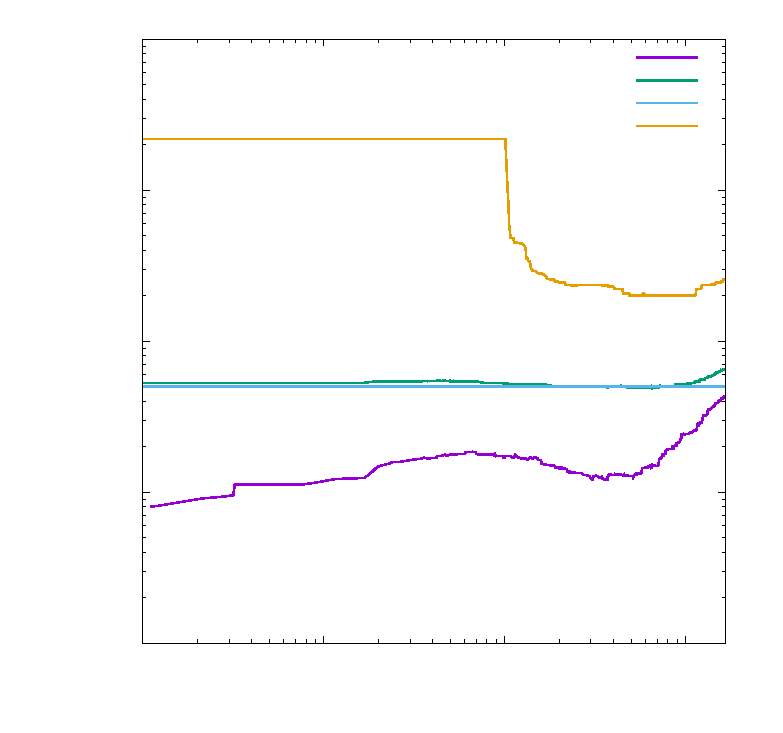
\includegraphics{con}}%
    \gplfronttext
  \end{picture}%
\endgroup
}
  \end{center}
  \caption{Estimating constant population size. For details see
  text.}\label{fig:con}
\end{figure}
\item Next, we simulate under the scenario used in Figure 2b of \cite{liu15:exp}
  with a single, approximately threefold change in population size
  from 7778 to 25636, which occurred 6809 generations ago:
\begin{verbatim}
mspms 30 1000 -t 12310 -r 9750 1e7 -eN 0.066 0.3 |
ms2sfs                                           |
epos -u 1.2e-8 -l 1e7 -U                         |
epos2plot > epos2.dat
\end{verbatim}
This again takes a few minutes.
\item Plot the result
\begin{verbatim}
gnuplot -p scripts/fig2.gp
\end{verbatim}
to get Figure~\ref{fig:2b}. The fit between the median estimated
population size and its true value remains excellent. However, the
variation in estimates is again large, particularly toward the present.
\begin{figure}
  \begin{center}
    \scalebox{0.6}{% GNUPLOT: LaTeX picture with Postscript
\begingroup
  \makeatletter
  \providecommand\color[2][]{%
    \GenericError{(gnuplot) \space\space\space\@spaces}{%
      Package color not loaded in conjunction with
      terminal option `colourtext'%
    }{See the gnuplot documentation for explanation.%
    }{Either use 'blacktext' in gnuplot or load the package
      color.sty in LaTeX.}%
    \renewcommand\color[2][]{}%
  }%
  \providecommand\includegraphics[2][]{%
    \GenericError{(gnuplot) \space\space\space\@spaces}{%
      Package graphicx or graphics not loaded%
    }{See the gnuplot documentation for explanation.%
    }{The gnuplot epslatex terminal needs graphicx.sty or graphics.sty.}%
    \renewcommand\includegraphics[2][]{}%
  }%
  \providecommand\rotatebox[2]{#2}%
  \@ifundefined{ifGPcolor}{%
    \newif\ifGPcolor
    \GPcolortrue
  }{}%
  \@ifundefined{ifGPblacktext}{%
    \newif\ifGPblacktext
    \GPblacktexttrue
  }{}%
  % define a \g@addto@macro without @ in the name:
  \let\gplgaddtomacro\g@addto@macro
  % define empty templates for all commands taking text:
  \gdef\gplbacktext{}%
  \gdef\gplfronttext{}%
  \makeatother
  \ifGPblacktext
    % no textcolor at all
    \def\colorrgb#1{}%
    \def\colorgray#1{}%
  \else
    % gray or color?
    \ifGPcolor
      \def\colorrgb#1{\color[rgb]{#1}}%
      \def\colorgray#1{\color[gray]{#1}}%
      \expandafter\def\csname LTw\endcsname{\color{white}}%
      \expandafter\def\csname LTb\endcsname{\color{black}}%
      \expandafter\def\csname LTa\endcsname{\color{black}}%
      \expandafter\def\csname LT0\endcsname{\color[rgb]{1,0,0}}%
      \expandafter\def\csname LT1\endcsname{\color[rgb]{0,1,0}}%
      \expandafter\def\csname LT2\endcsname{\color[rgb]{0,0,1}}%
      \expandafter\def\csname LT3\endcsname{\color[rgb]{1,0,1}}%
      \expandafter\def\csname LT4\endcsname{\color[rgb]{0,1,1}}%
      \expandafter\def\csname LT5\endcsname{\color[rgb]{1,1,0}}%
      \expandafter\def\csname LT6\endcsname{\color[rgb]{0,0,0}}%
      \expandafter\def\csname LT7\endcsname{\color[rgb]{1,0.3,0}}%
      \expandafter\def\csname LT8\endcsname{\color[rgb]{0.5,0.5,0.5}}%
    \else
      % gray
      \def\colorrgb#1{\color{black}}%
      \def\colorgray#1{\color[gray]{#1}}%
      \expandafter\def\csname LTw\endcsname{\color{white}}%
      \expandafter\def\csname LTb\endcsname{\color{black}}%
      \expandafter\def\csname LTa\endcsname{\color{black}}%
      \expandafter\def\csname LT0\endcsname{\color{black}}%
      \expandafter\def\csname LT1\endcsname{\color{black}}%
      \expandafter\def\csname LT2\endcsname{\color{black}}%
      \expandafter\def\csname LT3\endcsname{\color{black}}%
      \expandafter\def\csname LT4\endcsname{\color{black}}%
      \expandafter\def\csname LT5\endcsname{\color{black}}%
      \expandafter\def\csname LT6\endcsname{\color{black}}%
      \expandafter\def\csname LT7\endcsname{\color{black}}%
      \expandafter\def\csname LT8\endcsname{\color{black}}%
    \fi
  \fi
    \setlength{\unitlength}{0.0500bp}%
    \ifx\gptboxheight\undefined%
      \newlength{\gptboxheight}%
      \newlength{\gptboxwidth}%
      \newsavebox{\gptboxtext}%
    \fi%
    \setlength{\fboxrule}{0.5pt}%
    \setlength{\fboxsep}{1pt}%
\begin{picture}(7200.00,6720.00)%
    \gplgaddtomacro\gplbacktext{%
      \csname LTb\endcsname%%
      \put(1078,704){\makebox(0,0)[r]{\strut{}\large $10^{3}$}}%
      \put(1078,2636){\makebox(0,0)[r]{\strut{}\large $10^{4}$}}%
      \put(1078,4567){\makebox(0,0)[r]{\strut{}\large $10^{5}$}}%
      \put(1078,6499){\makebox(0,0)[r]{\strut{}\large $10^{6}$}}%
      \put(1389,484){\makebox(0,0){\strut{}\large $10^{-1}$}}%
      \put(2361,484){\makebox(0,0){\strut{}\large $10^{0}$}}%
      \put(3333,484){\makebox(0,0){\strut{}\large $10^{1}$}}%
      \put(4305,484){\makebox(0,0){\strut{}\large $10^{2}$}}%
      \put(5277,484){\makebox(0,0){\strut{}\large $10^{3}$}}%
      \put(6249,484){\makebox(0,0){\strut{}\large $10^{4}$}}%
    }%
    \gplgaddtomacro\gplfronttext{%
      \csname LTb\endcsname%%
      \put(198,3601){\rotatebox{-270}{\makebox(0,0){\strut{}\large $N_{\rm e}$}}}%
      \put(4006,154){\makebox(0,0){\strut{}\large Time (Generations)}}%
      \csname LTb\endcsname%%
      \put(5816,6326){\makebox(0,0)[r]{\strut{}\large 5\% quantile}}%
      \csname LTb\endcsname%%
      \put(5816,6106){\makebox(0,0)[r]{\strut{}\large median}}%
      \csname LTb\endcsname%%
      \put(5816,5886){\makebox(0,0)[r]{\strut{}\large 95\% quantile}}%
    }%
    \gplbacktext
    \put(0,0){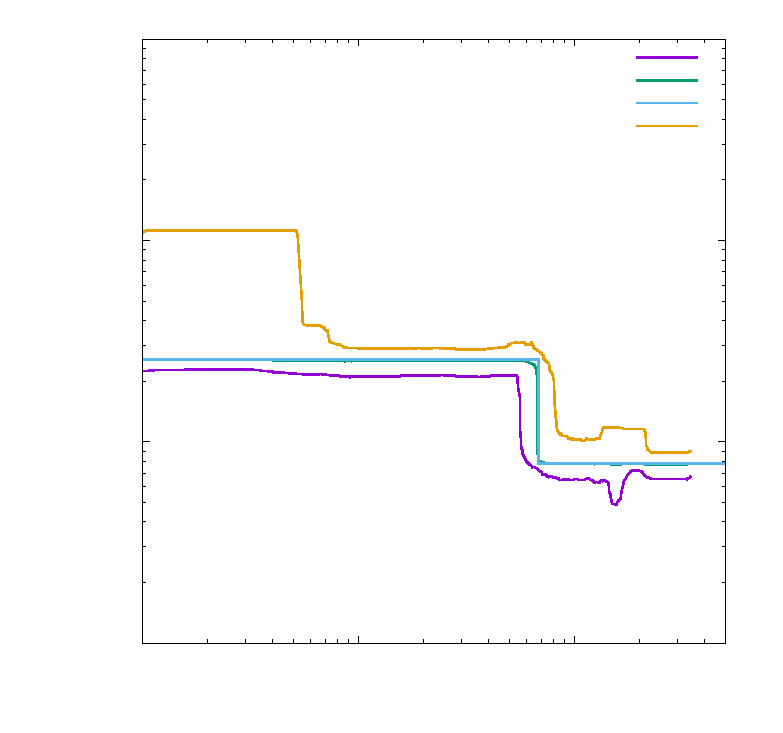
\includegraphics{fig2b}}%
    \gplfronttext
  \end{picture}%
\endgroup
}
  \end{center}
  \caption{Estimating population sizes under a model with one
    instantaneous size change. See text for details.}\label{fig:2b}
\end{figure}
\item As a last example, simulate haplotypes under
  the exponential growth scenario \cite{liu15:exp} used in their
  Figure 2e:
    \small
\begin{verbatim}
mspms 30 1000 -t 432000 -r 340000 1e7 -G 46368 -eN 0.0001027 0.008889 |
ms2sfs                                                                |
epos -u 1.2e-8 -l 1e7 -U                                              |
epos2plot > epos3.dat
\end{verbatim}
\normalsize
Plot this
\begin{verbatim}
gnuplot -p fig3.gp
\end{verbatim}
to get Figure~\ref{fig:2e}, where the estimation is precise until very
close to the present, when it starts to diverge. This illustrates
the difficulty of accurately calculating population size changes
in the recent past.
\begin{figure}
  \begin{center}
    \scalebox{0.6}{% GNUPLOT: LaTeX picture with Postscript
\begingroup
  \makeatletter
  \providecommand\color[2][]{%
    \GenericError{(gnuplot) \space\space\space\@spaces}{%
      Package color not loaded in conjunction with
      terminal option `colourtext'%
    }{See the gnuplot documentation for explanation.%
    }{Either use 'blacktext' in gnuplot or load the package
      color.sty in LaTeX.}%
    \renewcommand\color[2][]{}%
  }%
  \providecommand\includegraphics[2][]{%
    \GenericError{(gnuplot) \space\space\space\@spaces}{%
      Package graphicx or graphics not loaded%
    }{See the gnuplot documentation for explanation.%
    }{The gnuplot epslatex terminal needs graphicx.sty or graphics.sty.}%
    \renewcommand\includegraphics[2][]{}%
  }%
  \providecommand\rotatebox[2]{#2}%
  \@ifundefined{ifGPcolor}{%
    \newif\ifGPcolor
    \GPcolortrue
  }{}%
  \@ifundefined{ifGPblacktext}{%
    \newif\ifGPblacktext
    \GPblacktexttrue
  }{}%
  % define a \g@addto@macro without @ in the name:
  \let\gplgaddtomacro\g@addto@macro
  % define empty templates for all commands taking text:
  \gdef\gplbacktext{}%
  \gdef\gplfronttext{}%
  \makeatother
  \ifGPblacktext
    % no textcolor at all
    \def\colorrgb#1{}%
    \def\colorgray#1{}%
  \else
    % gray or color?
    \ifGPcolor
      \def\colorrgb#1{\color[rgb]{#1}}%
      \def\colorgray#1{\color[gray]{#1}}%
      \expandafter\def\csname LTw\endcsname{\color{white}}%
      \expandafter\def\csname LTb\endcsname{\color{black}}%
      \expandafter\def\csname LTa\endcsname{\color{black}}%
      \expandafter\def\csname LT0\endcsname{\color[rgb]{1,0,0}}%
      \expandafter\def\csname LT1\endcsname{\color[rgb]{0,1,0}}%
      \expandafter\def\csname LT2\endcsname{\color[rgb]{0,0,1}}%
      \expandafter\def\csname LT3\endcsname{\color[rgb]{1,0,1}}%
      \expandafter\def\csname LT4\endcsname{\color[rgb]{0,1,1}}%
      \expandafter\def\csname LT5\endcsname{\color[rgb]{1,1,0}}%
      \expandafter\def\csname LT6\endcsname{\color[rgb]{0,0,0}}%
      \expandafter\def\csname LT7\endcsname{\color[rgb]{1,0.3,0}}%
      \expandafter\def\csname LT8\endcsname{\color[rgb]{0.5,0.5,0.5}}%
    \else
      % gray
      \def\colorrgb#1{\color{black}}%
      \def\colorgray#1{\color[gray]{#1}}%
      \expandafter\def\csname LTw\endcsname{\color{white}}%
      \expandafter\def\csname LTb\endcsname{\color{black}}%
      \expandafter\def\csname LTa\endcsname{\color{black}}%
      \expandafter\def\csname LT0\endcsname{\color{black}}%
      \expandafter\def\csname LT1\endcsname{\color{black}}%
      \expandafter\def\csname LT2\endcsname{\color{black}}%
      \expandafter\def\csname LT3\endcsname{\color{black}}%
      \expandafter\def\csname LT4\endcsname{\color{black}}%
      \expandafter\def\csname LT5\endcsname{\color{black}}%
      \expandafter\def\csname LT6\endcsname{\color{black}}%
      \expandafter\def\csname LT7\endcsname{\color{black}}%
      \expandafter\def\csname LT8\endcsname{\color{black}}%
    \fi
  \fi
    \setlength{\unitlength}{0.0500bp}%
    \ifx\gptboxheight\undefined%
      \newlength{\gptboxheight}%
      \newlength{\gptboxwidth}%
      \newsavebox{\gptboxtext}%
    \fi%
    \setlength{\fboxrule}{0.5pt}%
    \setlength{\fboxsep}{1pt}%
\begin{picture}(7200.00,6720.00)%
    \gplgaddtomacro\gplbacktext{%
      \csname LTb\endcsname%%
      \put(1078,704){\makebox(0,0)[r]{\strut{}\large $10^{3}$}}%
      \put(1078,2636){\makebox(0,0)[r]{\strut{}\large $10^{4}$}}%
      \put(1078,4567){\makebox(0,0)[r]{\strut{}\large $10^{5}$}}%
      \put(1078,6499){\makebox(0,0)[r]{\strut{}\large $10^{6}$}}%
      \put(1210,484){\makebox(0,0){\strut{}\large $10^{0}$}}%
      \put(2445,484){\makebox(0,0){\strut{}\large $10^{1}$}}%
      \put(3679,484){\makebox(0,0){\strut{}\large $10^{2}$}}%
      \put(4914,484){\makebox(0,0){\strut{}\large $10^{3}$}}%
      \put(6148,484){\makebox(0,0){\strut{}\large $10^{4}$}}%
    }%
    \gplgaddtomacro\gplfronttext{%
      \csname LTb\endcsname%%
      \put(198,3601){\rotatebox{-270}{\makebox(0,0){\strut{}\large $N_{\rm e}$}}}%
      \put(4006,154){\makebox(0,0){\strut{}\large Time (Generations)}}%
      \csname LTb\endcsname%%
      \put(5816,6326){\makebox(0,0)[r]{\strut{}\large 5\% quantile}}%
      \csname LTb\endcsname%%
      \put(5816,6106){\makebox(0,0)[r]{\strut{}\large median}}%
      \csname LTb\endcsname%%
      \put(5816,5886){\makebox(0,0)[r]{\strut{}\large expected}}%
      \csname LTb\endcsname%%
      \put(5816,5666){\makebox(0,0)[r]{\strut{}\large 95\% quantile}}%
    }%
    \gplbacktext
    \put(0,0){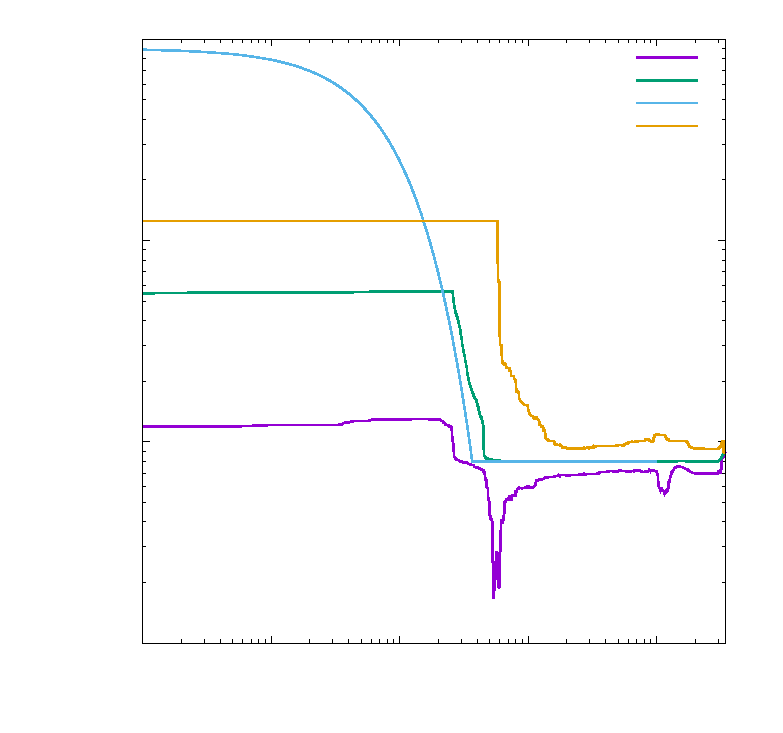
\includegraphics{fig2e}}%
    \gplfronttext
  \end{picture}%
\endgroup
}
  \end{center}
  \caption{Estimating population sizes under an exponential growth
    model. See text for details.}\label{fig:2e}
\end{figure}
\end{itemize}

\subsubsection*{Real Data}
I analyze the two site frequency spectra distributed with
\ty{epos}. One is from a population of water flea, \textit{Daphnia
  pulex}, the other from a human population, the Yoruba, who live in
south-western Nigeria. The \textit{Daphnia} data is provided by Mike
Lynch (Arizona State University), the Yoruba spectrum was computed by
\cite{lap17:acc} from the 1000 human genomes project data.
\paragraph{\textit{Daphnia pulex}}
\begin{itemize}
\item As an example for real data, we use a site frequency spectrum obtained from
  the Kap population of \textit{Daphnia pulex}:
\begin{verbatim}
head data/kap144i.dat 
0	185297
1	1987
2	1138
3	851
4	729
5	672
6	542
7	509
8	459
9	430
\end{verbatim}
Notice the ``zero-class'', which does not appear in the example
spectra in Tables~\ref{tab:sfs}A and B. The zero-class gives the
number of monomorphic sites. If a spectrum contains a zero-class, the
sequence length is the sum of all allele counts, and \ty{epos} does not
require the sequence length to be passed via the \ty{-l}
option. Moreover, the site frequency spectrum of Kap is folded, hence
no \ty{-U}:
\begin{verbatim}
epos data/kap144i.dat 
#InputFile: data/kap144i.dat
#Polymorphic sites surveyed:      18098
#Monomorphic sites surveyed:     185297
#m = 1; maximum Log(Likelihood):    -973.298394 {2}
#m = 2; maximum Log(Likelihood):    -306.995057 {2,24}
#m = 3; maximum Log(Likelihood):    -304.105038 {2,3,24}
#m = 4; maximum Log(Likelihood):    -297.264486 {2,3,8,24}
#m = 5; maximum Log(Likelihood):    -297.158028 {2,3,8,24,55}
#Final Log(Likelihood):             -297.264486
#d^2: 0.0039003
#Level  T[Level]        N[Level]
24      5.75e+04        3.93e+05
8       3.73e+05        7.94e+05
3       2.98e+06        1.82e+06
2       3.13e+06        7.89e+04                              
\end{verbatim}
\item A classical problem when estimating model parameters is
  ``over-fitting''. This refers to the fact that random quirks of a
  data set can strongly influence the estimation and hence
  generate a result specific to the particular data set but misleading
  with respect to the underlying population. We avoid over-fitting by
  requiring that a new level improves the log-likelihood of the model
  by at least 2 units (Algorithm~\ref{alg:epo}). A popular alternative is $k$-fold
  cross-validation \citep[p. 118f]{goo16:dee}. We can invoke this
  procedure with $k=5$, a typical value, using
\begin{verbatim}
epos -k 5 data/kap144i.dat 
...
#Final Log(Likelihood):             -297.30
#d^2: 0.003906
#Level  T[Level]        N[Level]
26      4.97e+04        3.76e+05
24      8.78e+04        2.74e+06
6       4.40e+05        5.63e+05
4       2.64e+06        4.12e+06
2       3.05e+06        1.55e+05
\end{verbatim}
which is very similar to the result with the log-likelihood threshold.
\item In many empirical data sets singletons are regarded as
  unreliable. To ignore singletons,
\begin{verbatim}
epos -x 1 data/kap144i.dat 
...
#Final Log(Likelihood):             -309.175057
#d^2: 0.00546917
#Level  T[Level]        N[Level]
29      3.37e+04        2.93e+05
2       3.94e+06        1.01e+06
\end{verbatim}
To ignore singletons and doubletons,
\begin{verbatim}
epos -x 1,2 data/kap144i.dat 
#InputFile: data/kap144i.dat
#Polymorphic sites surveyed:      14973
#Monomorphic sites surveyed:     185297
#m = 1; maximum Log(Likelihood):    -543.807666 {2}
#m = 2; maximum Log(Likelihood):    -310.507644 {2,39}
#m = 3; no improvement
#Final Log(Likelihood):             -310.507644
#d^2: 0.00634133
#Level  T[Level]        N[Level]
39      7.75e-02        1.00e+00
2       3.92e+06        1.01e+06
\end{verbatim}
which does not look like a very convincing result.
\item A run of \ty{epos} only gives a single point estimate,
  and in the absence of further samples it is hard to judge its
  reliability. However, the program \ty{bootSfs}, which is also part
  of the \ty{sfs} package bootstraps site frequency spectra to assess the
  robustness of results based on single samples. To run 1000 bootstrap
  replicates, enter
\begin{verbatim}
bootSfs -i 1000 kap144i.dat | epos | epos2plot > epos4.dat
\end{verbatim}
which takes about five minutes. Plot the result
\begin{verbatim}
gnuplot -p fig4.gp
\end{verbatim}
to get Figure~\ref{fig:kap}.
\begin{figure}
  \begin{center}
    \scalebox{0.6}{% GNUPLOT: LaTeX picture with Postscript
\begingroup
  \makeatletter
  \providecommand\color[2][]{%
    \GenericError{(gnuplot) \space\space\space\@spaces}{%
      Package color not loaded in conjunction with
      terminal option `colourtext'%
    }{See the gnuplot documentation for explanation.%
    }{Either use 'blacktext' in gnuplot or load the package
      color.sty in LaTeX.}%
    \renewcommand\color[2][]{}%
  }%
  \providecommand\includegraphics[2][]{%
    \GenericError{(gnuplot) \space\space\space\@spaces}{%
      Package graphicx or graphics not loaded%
    }{See the gnuplot documentation for explanation.%
    }{The gnuplot epslatex terminal needs graphicx.sty or graphics.sty.}%
    \renewcommand\includegraphics[2][]{}%
  }%
  \providecommand\rotatebox[2]{#2}%
  \@ifundefined{ifGPcolor}{%
    \newif\ifGPcolor
    \GPcolortrue
  }{}%
  \@ifundefined{ifGPblacktext}{%
    \newif\ifGPblacktext
    \GPblacktexttrue
  }{}%
  % define a \g@addto@macro without @ in the name:
  \let\gplgaddtomacro\g@addto@macro
  % define empty templates for all commands taking text:
  \gdef\gplbacktext{}%
  \gdef\gplfronttext{}%
  \makeatother
  \ifGPblacktext
    % no textcolor at all
    \def\colorrgb#1{}%
    \def\colorgray#1{}%
  \else
    % gray or color?
    \ifGPcolor
      \def\colorrgb#1{\color[rgb]{#1}}%
      \def\colorgray#1{\color[gray]{#1}}%
      \expandafter\def\csname LTw\endcsname{\color{white}}%
      \expandafter\def\csname LTb\endcsname{\color{black}}%
      \expandafter\def\csname LTa\endcsname{\color{black}}%
      \expandafter\def\csname LT0\endcsname{\color[rgb]{1,0,0}}%
      \expandafter\def\csname LT1\endcsname{\color[rgb]{0,1,0}}%
      \expandafter\def\csname LT2\endcsname{\color[rgb]{0,0,1}}%
      \expandafter\def\csname LT3\endcsname{\color[rgb]{1,0,1}}%
      \expandafter\def\csname LT4\endcsname{\color[rgb]{0,1,1}}%
      \expandafter\def\csname LT5\endcsname{\color[rgb]{1,1,0}}%
      \expandafter\def\csname LT6\endcsname{\color[rgb]{0,0,0}}%
      \expandafter\def\csname LT7\endcsname{\color[rgb]{1,0.3,0}}%
      \expandafter\def\csname LT8\endcsname{\color[rgb]{0.5,0.5,0.5}}%
    \else
      % gray
      \def\colorrgb#1{\color{black}}%
      \def\colorgray#1{\color[gray]{#1}}%
      \expandafter\def\csname LTw\endcsname{\color{white}}%
      \expandafter\def\csname LTb\endcsname{\color{black}}%
      \expandafter\def\csname LTa\endcsname{\color{black}}%
      \expandafter\def\csname LT0\endcsname{\color{black}}%
      \expandafter\def\csname LT1\endcsname{\color{black}}%
      \expandafter\def\csname LT2\endcsname{\color{black}}%
      \expandafter\def\csname LT3\endcsname{\color{black}}%
      \expandafter\def\csname LT4\endcsname{\color{black}}%
      \expandafter\def\csname LT5\endcsname{\color{black}}%
      \expandafter\def\csname LT6\endcsname{\color{black}}%
      \expandafter\def\csname LT7\endcsname{\color{black}}%
      \expandafter\def\csname LT8\endcsname{\color{black}}%
    \fi
  \fi
    \setlength{\unitlength}{0.0500bp}%
    \ifx\gptboxheight\undefined%
      \newlength{\gptboxheight}%
      \newlength{\gptboxwidth}%
      \newsavebox{\gptboxtext}%
    \fi%
    \setlength{\fboxrule}{0.5pt}%
    \setlength{\fboxsep}{1pt}%
\begin{picture}(7200.00,6720.00)%
    \gplgaddtomacro\gplbacktext{%
      \csname LTb\endcsname%%
      \put(1078,704){\makebox(0,0)[r]{\strut{}\large $10^{4}$}}%
      \put(1078,2153){\makebox(0,0)[r]{\strut{}\large $10^{5}$}}%
      \put(1078,3601){\makebox(0,0)[r]{\strut{}\large $10^{6}$}}%
      \put(1078,5050){\makebox(0,0)[r]{\strut{}\large $10^{7}$}}%
      \put(1078,6499){\makebox(0,0)[r]{\strut{}\large $10^{8}$}}%
      \put(2756,484){\makebox(0,0){\strut{}\large $10^{4}$}}%
      \put(4308,484){\makebox(0,0){\strut{}\large $10^{5}$}}%
      \put(5860,484){\makebox(0,0){\strut{}\large $10^{6}$}}%
    }%
    \gplgaddtomacro\gplfronttext{%
      \csname LTb\endcsname%%
      \put(198,3601){\rotatebox{-270}{\makebox(0,0){\strut{}\large $N_{\rm e}$}}}%
      \put(4006,154){\makebox(0,0){\strut{}\large Time (Generations)}}%
      \csname LTb\endcsname%%
      \put(5816,6326){\makebox(0,0)[r]{\strut{}\large 5\% quantile}}%
      \csname LTb\endcsname%%
      \put(5816,6106){\makebox(0,0)[r]{\strut{}\large median}}%
      \csname LTb\endcsname%%
      \put(5816,5886){\makebox(0,0)[r]{\strut{}\large 95\% quantile}}%
    }%
    \gplbacktext
    \put(0,0){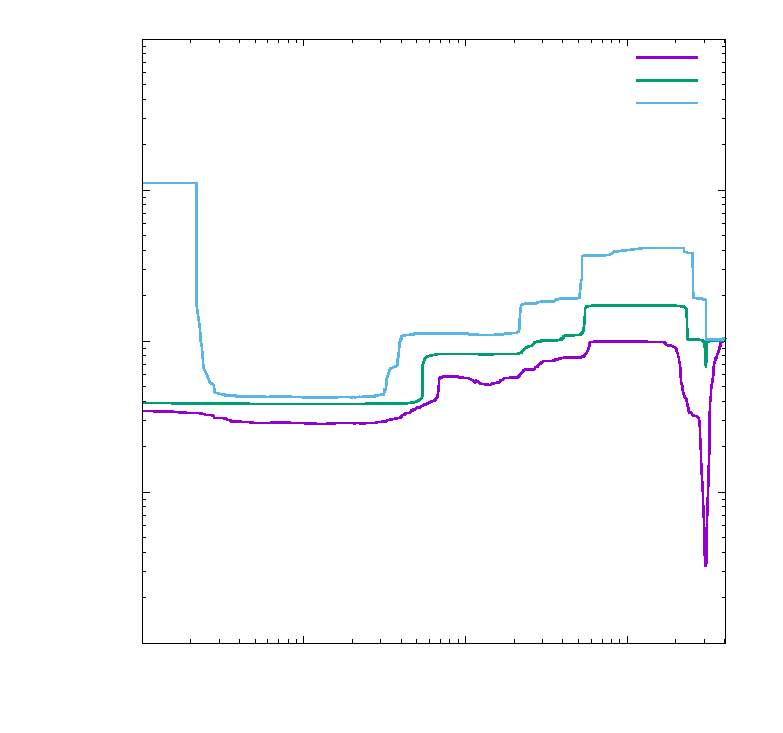
\includegraphics{kap}}%
    \gplfronttext
  \end{picture}%
\endgroup
}
  \end{center}
  \caption{Estimating the population size of the \textit{D. pulex} Kap
    population.}\label{fig:kap}
\end{figure}
\end{itemize}

\paragraph{The Yoruba Population}
\begin{itemize}
\item Analyze the full spectrum:
\begin{verbatim}
epos -u 1.2e-8 -l 2.9e9 data/FoldSFS_YRI.txt 
#InputFile: data/FoldSFS_YRI.txt
#Polymorphic sites surveyed:   20440078
#Monomorphic sites surveyed: 2879559922
...
#Final Log(Likelihood):            -1177.60
#d^2: 4.38702e-05
#Level  T[Level]        N[Level]
216     8.76e+01        1.02e+06
142     4.21e+02        3.41e+04
121     4.24e+02        6.75e+02
13      9.13e+03        2.90e+04
10      1.18e+04        2.43e+04
3       4.94e+04        2.42e+04
2       7.07e+04        1.06e+04
\end{verbatim}
where $\mu=1.2\times 10^{-8}$ is the mutation rate used by
\cite{lap17:acc} and $2.9\times 10^9$ the number of sequenced
nucleotides in the human genome.
\item \cite{lap17:acc} excluded
the singletons in their analysis. To do this in \ty{epos}, we rerun the analysis with
\ty{-x 1}
\begin{verbatim}
epos -x 1 -u 1.2e-8 -l 2.9e9 data/FoldSFS_YRI.txt 
#InputFile: data/FoldSFS_YRI.txt
#Polymorphic sites surveyed:   15937781
#Monomorphic sites surveyed: 2879559922
...
#Final Log(Likelihood):            -3132.160271
#d^2: 8.04994e-05
#Level  T[Level]        N[Level]
181     3.70e-03        1.00e+00
28      3.51e+03        2.79e+04
6       2.23e+04        2.88e+04
5       2.30e+04        3.59e+03
2       7.61e+04        1.77e+04
\end{verbatim}
\item As with the \textit{Daphnia} data, we can bootstrap the Youruba
  mutation spectrum. Figure~\ref{fig:yri}A shows the demography based on $10^4$
  bootstrap samples including all allele classes and assuming 24 years
  per generation. The apparent jump from $3\times 10^4$ to $10^6$
  approximately 2000 years ago is abolished by
  excluding singletons (Figure~\ref{fig:yri}B). In contrast, the
  baseline size of approximately $3\times 10^4$ remains unchanged. The bootstrap analysis
  including all mutation classes takes approximately 15 CPU hours, a
  bit less if singletons are excluded. Such massive run times are
  best managed by starting, say, 50 jobs with 200 resamplings on a
  multi-core machine. \ty{Epos} lends itself to this kind of
  pseudo-parallelization, as its memory consumption is only 4.3 MB per
  run on the Yoruba sample, which is negligible on current computers.
\end{itemize}

\begin{figure}
  \begin{center}
    \resizebox{\textwidth}{!}{
        \begin{tabular}{cc}
          \Large\textbf{A} & \Large\textbf{B}\\
          \input{yriSi} & \input{yriNoSi}
        \end{tabular}
    }
  \end{center}
  \caption{Analysis of the Yoruba site frequency spectrum including
    the singletons (\textbf{A}) and excluding them
    (\textbf{B}).}\label{fig:yri}
\end{figure}


\subsection{\ty{Epos2ages}}
The program \ty{epos2ages} converts population sizes computed by
\ty{epos} to average ages of alleles \citep{lyn19:inf}.
\begin{itemize}
  \item To start with a simple example, simulate a site frequency spectrum with $n=2$,
\begin{verbatim}
ms 2 1 -t 10 | ms2sfs > test.sfs
\end{verbatim}
estimate the population size,
\begin{verbatim}
epos -U -l 1000 test.sfs
#InputFile: test.sfs
#Polymorphic sites surveyed:         36
#Monomorphic sites surveyed:        964
#m = 1; maximum Log(Likelihood):      -7.07 {2}
#m = 2; no improvement
#Final Log(Likelihood):               -7.07
#d^2: 0
#Level	T[Level]	N[Level]
2	3.60e+06	1.80e+06
\end{verbatim}
and the age of singletons
\begin{verbatim}
epos -U -l 1000 test.sfs | epos2ages -n 2
#r  A[r]     V(A[r])    P[r]
1   3.6e+06  1.296e+13  1.8e+06
\end{verbatim}
where the second column gives their average age as $3\times 10^6$,
twice the population size. Since \ty{epos2ages} follows the convention
of measuring time in units of $2N$ generations, this is the correct
result. The other two output columns of \ty{epos2ages} are the
variance of the age, and the average population size experienced by
the allele, which again agrees with the previous \ty{epos} result.
\item For larger samples of 30 haplotypes the population sizes might look like this
\begin{verbatim}
ms 30 1 -t 1000 | ms2sfs | tee test.sfs | epos -U -l 1e7
#InputFile: stdin
#Polymorphic sites surveyed:       3055
#Monomorphic sites surveyed:    9996945
#m = 1; maximum Log(Likelihood):   -1520.427498 {2}
#m = 2; maximum Log(Likelihood):   -1162.883232 {2,4}
#m = 3; maximum Log(Likelihood):   -1156.803456 {2,4,16}
#m = 4; no improvement
#Final Log(Likelihood):            -1156.803456
#d^2: 1.13251
#Level  T[Level]        N[Level]
16      6.08e+02        4.56e+03
4       8.24e+03        7.15e+03
2       8.24e+03        1.00e+00
\end{verbatim}
and the corresponding allele sizes
\begin{verbatim}
epos -U -l 1e7 test.sfs | epos2ages -n 30
#r      A[r]    V(A[r])         P[r]
1       1713.61 5.28278e+06     6467.4
2       2602.4  7.05225e+06     6596.96
3       3236.13 8.04631e+06     6678.69
...
29      8237.33	9.83744e+06	6956.52
\end{verbatim}
\item Finally, we can estimate the average age of alleles for the Kap
  population:
\begin{verbatim}
epos2ages -n 144 data/kap144i.out
#r      A[r]    V(A[r])      P[r]
1       232151  4.18264e+11  1.38013e+06
2       382824  6.51857e+11  1.4013e+06
3       493525  8.05644e+11  1.41684e+06
...
143     3.13086e+06  2.09611e+12  1.60264e+06
\end{verbatim}  
\end{itemize}

\section{Change Log}
The change log can be accessed via the repository web page
\begin{verbatim}
https://github.com/evolbioinf/epos
\end{verbatim}
or inside a local copy of the repository by executing
\begin{verbatim}
git log
\end{verbatim}

\bibliography{ref}
\end{document}

